\section{Results}\label{sec:results}

\subsection{Accuracy of multi-source forecasts (RQ1)}
Table~\ref{tab:models} and Fig.~\ref{fig:models} summarise the 1{,}600 test forecasts. Climatology reached an RMSE of \rmseClim~\kgrai{} and persistence \rmsePers~\kgrai. Every multi-source learner was more accurate. LightGBM had the lowest test error (\rmseLGB~\kgrai, i.e.\ \thaLGB~t\,ha$^{-1}$; MAPE \mapeLGB\%), \redClimLGBPct\% below climatology, followed by the random forest (\rmseRF) and the validation-selected ensemble (\rmseMain~\kgrai; 95\% CI \rmseLoMain--\rmseHiMain), which reduced the climatology error by \redClimPct\% (difference \drmseClim~\kgrai, CI \drmseLoClim--\drmseHiClim). The multilayer perceptron (\rmseMLP), the panel fixed-effects model (\rmseFE) and Ridge regression (\rmseRidge) were less accurate. The skill measures confirm that the gains concern the season-to-season deviations that matter for forecasting: LightGBM explained a share of \rtwoanomLGB{} of the variance of the anomaly relative to the previous-three-season mean (Skill \skillLGB), the ensemble \rtwoanomMain{} (Skill \skillMain).

Formal tests were less conclusive than these magnitudes suggest. With only eight test seasons and Holm adjustment over eight comparisons, no Diebold--Mariano test against the ensemble was significant at the 5\% level (smallest adjusted $p=\dmpPers$, for persistence; $p=\dmpClim$ for climatology). The season-bootstrap interval of the ensemble's advantage over climatology nevertheless excludes zero, and the replicate worlds (Section~\ref{sec:res-robust}) show that the advantage is systematic.

Model selection on the validation seasons favoured the ensemble (validation RMSE \valRmseEns, against \valRmseRidge{} for Ridge and \valRmseLGB{} for LightGBM), but on the test seasons LightGBM was more accurate (RMSE difference $\drmseLGB$~\kgrai, 95\% CI $\drmseLoLGB$ to $\drmseHiLGB$). The error by season (Fig.~\ref{fig:seasons}) shows why: the linear learners failed in single seasons---Ridge in \worstYearRidge{} (RMSE \worstRidge) and the panel model in \worstYearFE{} (\worstFE)---and the ensemble inherited half of Ridge's failure (\worstEns{} in \worstYearEns), whereas LightGBM never exceeded \worstLGB~\kgrai{} in any season. In the remaining seasons the ensemble was usually the most accurate learner, including the shock seasons \shockYears, in which climatology and persistence were worst. The level target was preferred to the anomaly target during tuning, and the anomaly-target LightGBM was also less accurate on the test seasons (\rmseLGBalt).

\begin{figure}[t]\centering
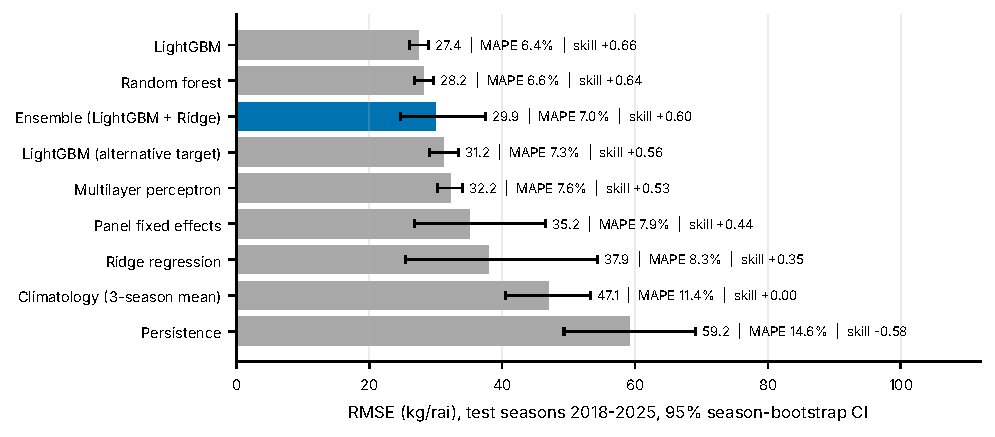
\includegraphics[width=\textwidth]{fig3_model_comparison}
\caption{Test RMSE of the eight learners (rolling origin, 2018--2025) with 95\% season-block bootstrap intervals; the validation-selected main model is highlighted. Text: RMSE, MAPE and skill relative to climatology.}\label{fig:models}
\end{figure}

\begin{table}[t]\centering\scriptsize
\caption{Out-of-sample accuracy on the test seasons 2018--2025 (rolling origin; 1{,}600 district-season forecasts). RMSE and MAE in kg\,rai$^{-1}$ (multiply by 0.00625 for t\,ha$^{-1}$); brackets: 95\% season-block bootstrap CI. $R^2_{\mathrm{anom}}$: skill on deviations from the previous-3-season mean; Skill: $1-\mathrm{MSE}/\mathrm{MSE}_{\mathrm{clim}}$. $p_{\mathrm{DM}}$: Holm-adjusted Diebold--Mariano (HLN) test against the main model ($^{\star}$).}\label{tab:models}
\begin{tabular}{@{}lccccccc@{}}
\toprule
Model & RMSE [95\% CI] & MAE & MAPE (\%) & $R^2$ & $R^2_{\mathrm{anom}}$ & Skill & $p_{\mathrm{DM}}$ \\
\midrule
LightGBM & 27.4 [26.1, 29.0] & 21.7 & 6.4 & 0.89 & 0.66 & +0.66 & 1.000 \\
Random forest & 28.2 [26.8, 29.6] & 22.2 & 6.6 & 0.88 & 0.64 & +0.64 & 1.000 \\
Ensemble (LightGBM + Ridge) $^{\star}$ & 29.9 [24.7, 37.4] & 23.4 & 7.0 & 0.87 & 0.59 & +0.60 & -- \\
LightGBM (alternative target) & 31.2 [29.0, 33.4] & 24.6 & 7.3 & 0.85 & 0.56 & +0.56 & 1.000 \\
Multilayer perceptron & 32.2 [30.3, 34.0] & 25.6 & 7.6 & 0.84 & 0.53 & +0.53 & 1.000 \\
Panel fixed effects & 35.2 [26.8, 46.5] & 27.5 & 7.9 & 0.81 & 0.44 & +0.44 & 1.000 \\
Ridge regression & 37.9 [25.4, 54.3] & 27.9 & 8.3 & 0.78 & 0.35 & +0.35 & 1.000 \\
Climatology (3-season mean) & 47.1 [40.6, 53.2] & 37.8 & 11.4 & 0.67 & -0.00 & +0.00 & 0.251 \\
Persistence & 59.2 [49.3, 69.1] & 48.1 & 14.6 & 0.47 & -0.59 & -0.58 & 0.080 \\
\bottomrule
\end{tabular}
\end{table}

\begin{figure}[t]\centering
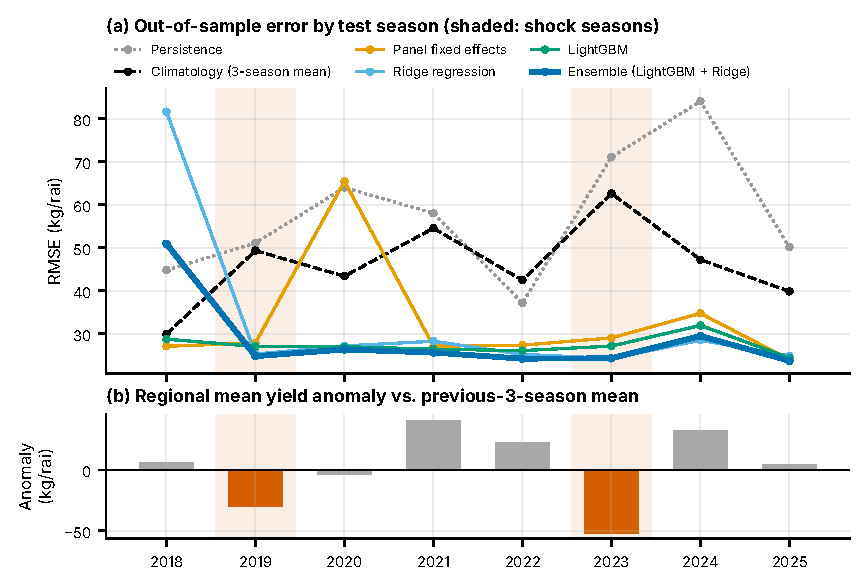
\includegraphics[width=\textwidth]{fig4_error_by_season}
\caption{(a) RMSE by test season. The linear learners fail in single seasons (Ridge in \worstYearRidge, panel fixed effects in \worstYearFE), and the ensemble inherits part of Ridge's failure. (b) Regional mean yield anomaly relative to the previous-three-season mean; shaded seasons are shock seasons (anomaly more than one standard deviation below the mean of all seasons).}\label{fig:seasons}
\end{figure}

\subsection{Leakage inflates apparent skill and hides failures (RQ2)}
Table~\ref{tab:leakage} and Fig.~\ref{fig:leakage} compare the leakage-safe estimates with four flawed protocols. For LightGBM---the learner whose honest performance was stable---random 5-fold cross-validation understated the RMSE by \gainRandomLGB\%, and adding the neighbours' current-season yields by \gainNbrLGB\%. Anomalies computed against the full-period mean had a negligible effect (\gainFutureLGB\%), and same-season prices did not help ($\gainPriceLGB$\%) although they carry information about the current harvest through the price feedback; a plausible explanation is that, with fewer than fifteen training seasons, a predictor that varies mainly between seasons is hard to exploit. Apparent gains were much larger for Ridge and the ensemble (random cross-validation: \gainRandomRidge\% and \gainRandom\%), but for a different reason: under the flawed protocols the linear learner no longer had to extrapolate to an unseen season, and its catastrophic failure disappeared. Random cross-validation therefore did not merely inflate skill; it concealed the failure mode altogether. The replicate worlds confirm the pattern: the randomly cross-validated ensemble reported \repRandomCV~$\pm$~\repSdRandomCV~\kgrai{} in every world (range \repMinRandomCV--\repMaxRandomCV), whereas its honest RMSE ranged from \repMinEns{} to \repMaxEns.

\begin{figure}[t]\centering
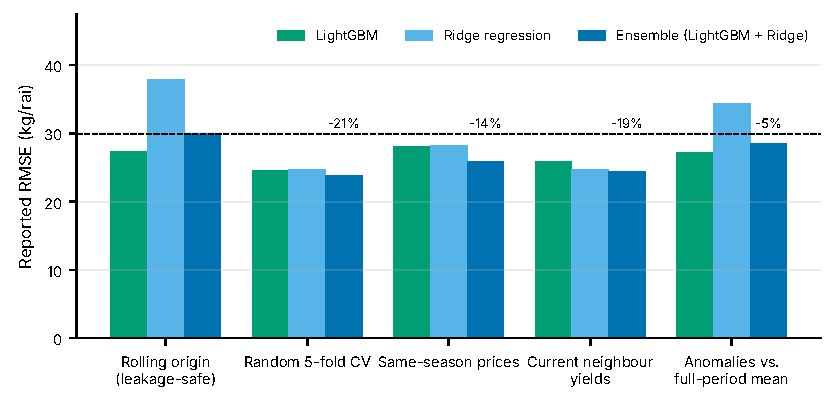
\includegraphics[width=\textwidth]{fig5_leakage}
\caption{Reported test RMSE under the leakage-safe rolling origin (dashed line: main model) and under four flawed protocols, all scored on the same 1{,}600 forecasts; labels give the change for the main model.}\label{fig:leakage}
\end{figure}

\begin{table}[t]\centering\footnotesize
\caption{Leakage audit: RMSE (kg\,rai$^{-1}$) reported on the same 1{,}600 test forecasts under the leakage-safe protocol and under four flawed protocols; parentheses: change relative to the leakage-safe RMSE (negative = optimistic bias).}\label{tab:leakage}
\begin{tabular}{@{}lccc@{}}
\toprule
Protocol & LightGBM & Ridge & Ensemble \\
\midrule
Rolling origin (leakage-safe) & 27.4 & 37.9 & 29.9 \\
Random 5-fold CV & 24.6 (-10\%) & 24.7 (-35\%) & 23.8 (-21\%) \\
Same-season prices & 28.0 (+2\%) & 28.3 (-25\%) & 25.9 (-14\%) \\
Current neighbour yields & 25.9 (-5\%) & 24.6 (-35\%) & 24.3 (-19\%) \\
Anomalies vs. full-period mean & 27.2 (-1\%) & 34.4 (-9\%) & 28.5 (-5\%) \\
\bottomrule
\end{tabular}
\end{table}

\subsection{Which predictors matter (RQ3)}
Drop-one-group ablation (Fig.~\ref{fig:attribution}a; Table~\ref{tab:ablation}) identified the satellite group as the only group whose removal materially degraded LightGBM (\ablLGBSatellite\%); removing any other group changed its RMSE by between $\ablLGBHistory$\% and $\ablLGBMap$\%. The weather, soil-moisture, price, terrain and history groups are therefore individually substitutable: much of their information is also contained in other groups---soil moisture in rainfall and LSWI, the district level in terrain, soils and neighbours' yields. For the ensemble, removing the satellite group raised the RMSE by \ablSatellite\% and removing geography by \ablGeography\%, but removing the moisture, climate or price features \emph{lowered} it ($\ablMoisture$\%, $\ablClimate$\% and $\ablPrice$\%), because every reduction of the season-level feature set reduced Ridge's scope for extrapolation. Ablation results of a fragile learner thus mix information content with model stability.

Grouped SHAP shares differed sharply between learners (Fig.~\ref{fig:attribution}b). LightGBM attributed \shapLGBSatellite\% of the mean absolute SHAP value to the satellite group, \shapLGBHistory\% to history and \shapLGBMoisture\% to moisture, but only \shapLGBPrice\% to prices. The ensemble attributed the largest share to prices (\shapPrice\%), followed by the satellite (\shapSatellite\%) and moisture (\shapMoisture\%) groups. Ablation and SHAP answer different questions---the marginal predictive value of a group versus its use by a particular model---and the ensemble's large price share reflects Ridge's use of season-level price variables rather than their predictive value, since removing them improved the ensemble. The satellite group's value is not restricted to pests: in the world without pest outbreaks the ensemble's RMSE still rose from \scenNoPestEns{} to \scenNoPestNoSat~\kgrai{} without satellite features, because canopy indices integrate the visible state of the crop, including drought, management and soil effects.

\begin{figure}[t]\centering
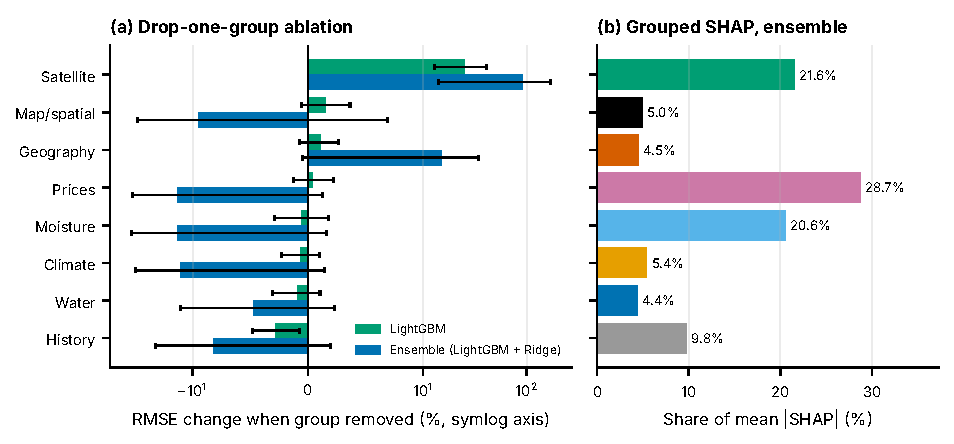
\includegraphics[width=\textwidth]{fig6_attribution}
\caption{(a) Change in test RMSE when a feature group is removed and the learner re-trained (95\% season-bootstrap intervals; symmetric-log axis). (b) Share of mean absolute SHAP values by group for the main model.}\label{fig:attribution}
\end{figure}

\subsection{Do explanations recover the true mechanisms? (RQ3)}
Because the simulator stores the true yield components, attributions can be checked directly (Fig.~\ref{fig:recovery}, Table~\ref{tab:recovery}). Two mechanisms were recovered well: the district base level, through the history, geography and map groups ($r=\recBase$ for the ensemble and \recLGBBase{} for LightGBM), and drought, through the moisture, water and satellite groups ($r=\recDrought$ and \recLGBDrought); the binned SHAP curve of the moisture and water groups reproduced the threshold response of the true drought component (Fig.~\ref{fig:dependence}a). Recovery failed in three characteristic ways. First, \emph{substitution among correlated mechanisms}: heat stress around flowering, which co-occurs with dry conditions, was credited mainly to the moisture and water groups, while the climate group's SHAP was negatively correlated with the true heat penalty ($r=\recHeat$; Fig.~\ref{fig:dependence}d). Second, \emph{absorption of season-level effects}: the technology trend, a pure season effect, was not recovered by the history group ($r=\recTrend$) but correlated strongly and negatively with the price group's SHAP (Fig.~\ref{fig:recovery}); a predictor that varies mainly between seasons can stand in for any season effect. Third, \emph{weak or diluted signals}: floods ($r=\recFlood$), humid-season disease ($r=\recDisease$) and management ($r=\recMgmt$) were essentially not recovered, and pest outbreaks only weakly ($r=\recPest$), partly because their satellite signal is shared with the neighbours' NDVI anomalies in the map group. Learner stability mattered most for prices: LightGBM's price and map attributions tracked the true price effect ($r=\recLGBPrice$), whereas the ensemble's did not ($r=\recPrice$), and its price SHAP even ran against the true response (Fig.~\ref{fig:dependence}c). Unobservable noise was, correctly, attributed to no group.

\begin{figure}[t]\centering
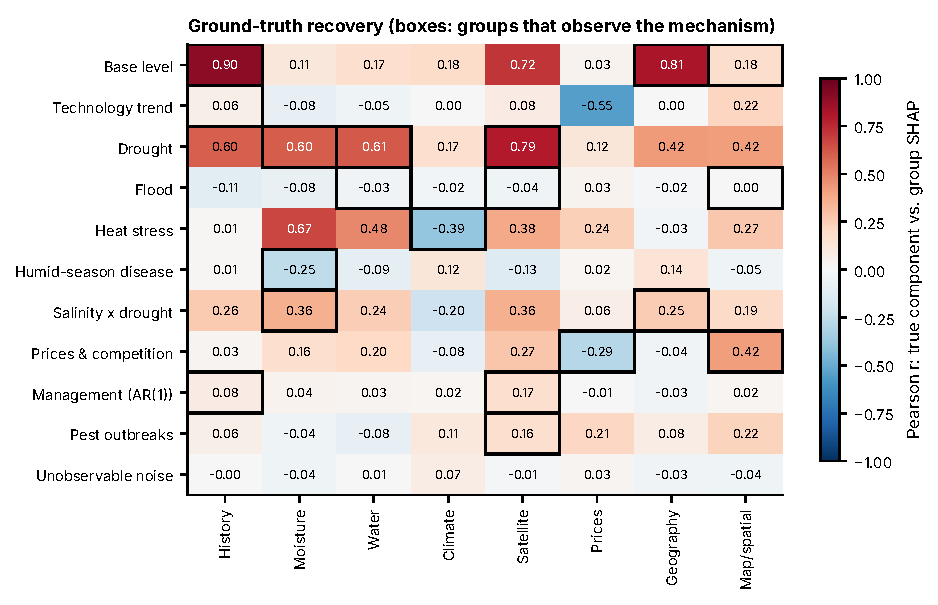
\includegraphics[width=\textwidth]{fig8_truth_recovery}
\caption{Correlation between each true yield component of the DGP and the summed SHAP values of each feature group (main model, 1{,}600 test forecasts). Boxes mark the groups that observe a mechanism; a faithful explanation would place large positive values in the boxes.}\label{fig:recovery}
\end{figure}

\begin{table}[t]\centering\footnotesize
\caption{Ground-truth recovery on the test forecasts. s.d.: standard deviation of the true component (kg\,rai$^{-1}$); $r_{\mathrm{obs}}$: Pearson correlation between the true component and the summed SHAP values of the groups that observe it, for the main model and (post hoc) for LightGBM alone; last column (main model): the single group whose SHAP correlates most strongly (absolute value) with the component.}\label{tab:recovery}
\begin{tabular}{@{}lcp{3.6cm}ccc@{}}
\toprule
True component & s.d. & Observed by & $r_{\mathrm{obs}}$ main & $r_{\mathrm{obs}}$ LightGBM & Best single group ($r$) \\
\midrule
Base level & 44.8 & Geography, Map/spatial, History & 0.90 & 0.92 & History (0.90) \\
Technology trend & 5.0 & History & 0.06 & 0.06 & Prices (-0.55) \\
Drought & 39.0 & Moisture, Water, Satellite & 0.84 & 0.88 & Satellite (0.79) \\
Flood & 5.4 & Water, Map/spatial, Satellite & -0.04 & -0.05 & History (-0.11) \\
Heat stress & 9.5 & Climate & -0.39 & -0.34 & Moisture (0.67) \\
Humid-season disease & 5.1 & Moisture & -0.25 & 0.00 & Moisture (-0.25) \\
Salinity $\times$ drought & 0.8 & Geography, Moisture & 0.41 & 0.33 & Satellite (0.36) \\
Prices \& competition & 14.4 & Prices, Map/spatial & -0.02 & 0.52 & Map/spatial (0.42) \\
Management (AR(1)) & 17.4 & History, Satellite & 0.14 & 0.14 & Satellite (0.17) \\
Pest outbreaks & 10.3 & Satellite & 0.16 & 0.16 & Map/spatial (0.22) \\
Unobservable noise & 15.9 & -- & -- & -- & Climate (0.07) \\
\bottomrule
\end{tabular}
\end{table}

\begin{figure}[t]\centering
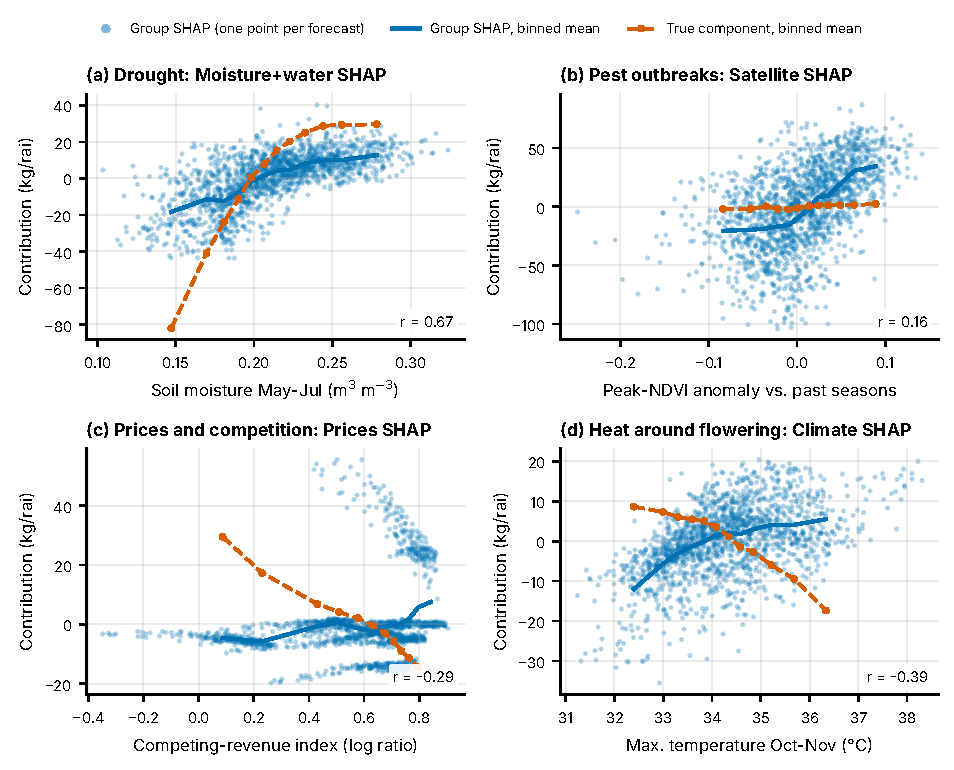
\includegraphics[width=\textwidth]{fig7_dependence_vs_truth}
\caption{Group SHAP values of the main model (points and solid line: binned mean) and the true component (dashed line: binned mean) along the main observed driver of four mechanisms; both are centred. $r$: correlation between group SHAP and true component.}\label{fig:dependence}
\end{figure}

\subsection{In-season forecasting (RQ4)}
LightGBM's RMSE fell from \leadLGBJul~\kgrai{} with data to the end of July to \leadLGBAug{} (August), \leadLGBSep{} (September), \leadLGBOct{} (October) and \leadLGBNov{} (November), and it was below climatology (\leadClim) at every forecast date (Fig.~\ref{fig:leadtime}a). The value of the satellite group was negligible until September (\satGainLGBJul, \satGainLGBAug{} and \satGainLGBSep~\kgrai) and became substantial once the canopy approached its peak (\satGainLGBOct{} in October and \satGainLGBNov{} in November; Fig.~\ref{fig:leadtime}b). Ridge, in contrast, was unusable early in the season (\leadRidgeJul~\kgrai{} in July), and the ensemble inherited this failure (\leadJul).

\begin{figure}[t]\centering
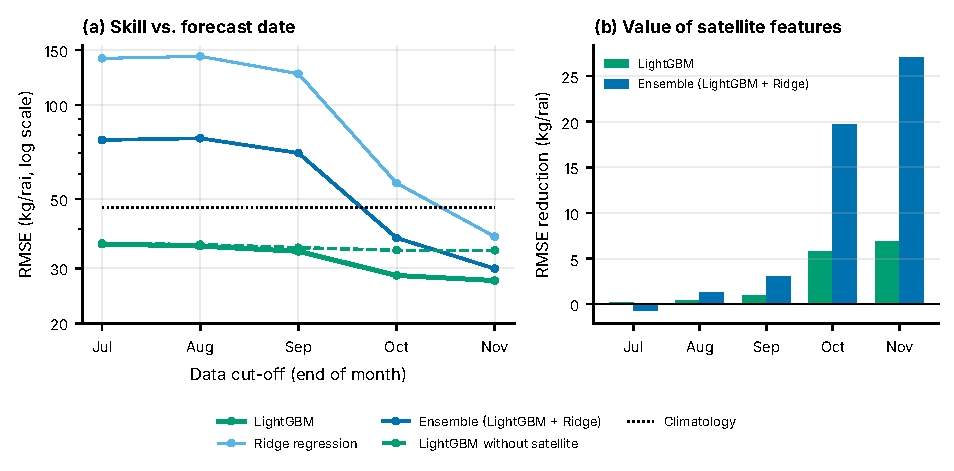
\includegraphics[width=\textwidth]{fig9_leadtime}
\caption{(a) Test RMSE as a function of the data cut-off month (log scale). (b) RMSE reduction contributed by the satellite group at each cut-off.}\label{fig:leadtime}
\end{figure}

\subsection{Calibration of prediction intervals (RQ4)}
Rolling split-conformal intervals of the main model were close to nominal: 80\% intervals covered \covEighty\% and 90\% intervals \covNinety\% of the test yields, with mean widths of \widthEighty{} and \widthNinety~\kgrai{} (Fig.~\ref{fig:conformal}). Contrary to H6, coverage was \emph{higher} in the shock seasons \shockYears{} (\covEightyShock\% and \covNinetyShock\%) than in the other seasons (\covEightyOther\% and \covNinetyOther\%): the drought shocks were well predicted because their causes are observed. Under-coverage was instead concentrated in the season of the model failure (\covEightyMin\% of 80\% intervals in \covEightyMinYear). Calibration on past errors thus protects against average miscalibration but not against a new failure mode of the point forecaster.

\begin{figure}[t]\centering
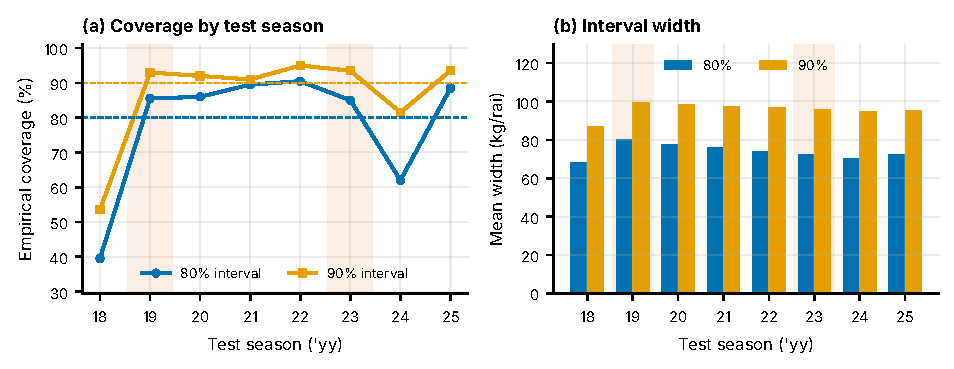
\includegraphics[width=\textwidth]{fig10_conformal}
\caption{Rolling split-conformal prediction intervals of the main model: (a) empirical coverage by test season (dashed: nominal levels; shaded: shock seasons); (b) mean interval width.}\label{fig:conformal}
\end{figure}

\subsection{Robustness across worlds and scenarios}\label{sec:res-robust}
Across ten independently simulated worlds (Table~\ref{tab:robust}), LightGBM was remarkably stable (RMSE \repLGB~$\pm$~\repSdLGB, range \repMinLGB--\repMaxLGB), while climatology reached \repClim~$\pm$~\repSdClim. The ensemble had the lowest median RMSE (\repMedEns) and beat LightGBM in \repWinsEnsLGB{} of \nRep{} worlds, but its mean (\repEns~$\pm$~\repSdEns) was inflated by \repFailEns{} failures (RMSE more than 1.5 times that of LightGBM), and Ridge failed in \repFailRidge{} worlds (median \repMedRidge, maximum \repMaxRidge). Without satellite features the ensemble's median RMSE rose to \repMedNoSat. In the scenario worlds LightGBM stayed between \scenNoPestLGB{} and \scenCloudsLGB~\kgrai, even under strong non-linearity (\scenNonlinLGB, against \scenNonlinClim{} for climatology), whereas Ridge degraded with non-linearity (\scenNonlinRidge), cloud contamination (\scenCloudsRidge) and map-layer error (\scenMapErrRidge). In the world without pest outbreaks the three learners performed similarly (ensemble \scenNoPestEns, Ridge \scenNoPestRidge, LightGBM \scenNoPestLGB).

\begin{table}[t]\centering\scriptsize
\caption{Robustness: test RMSE (kg\,rai$^{-1}$) in the main world, across ten independently simulated replicate worlds, and in four DGP scenarios (seed 42), with the configuration tuned once in the main world. ``No sat.'': ensemble without satellite features; ``Random CV'': the same ensemble scored with naive random 5-fold cross-validation.}\label{tab:robust}
\begin{tabular}{@{}lcccccc@{}}
\toprule
World & Climatology & Ridge & LightGBM & Ensemble & No sat. & Random CV \\
\midrule
Main world (seed 42) & 47.1 & 37.9 & 27.4 & 29.9 & 56.9 & 23.8 \\
Replicates, mean $\pm$ s.d. ($n=10$) & 49.4 $\pm$ 2.9 & 44.2 $\pm$ 28.6 & 26.5 $\pm$ 0.5 & 31.8 $\pm$ 11.4 & 38.5 $\pm$ 12.6 & 23.5 $\pm$ 0.4 \\
\midrule
Stronger non-linearity & 87.2 & 157.5 & 28.5 & 83.9 & 166.8 & 26.2 \\
3$\times$ map-layer error & 47.1 & 39.3 & 27.6 & 30.5 & 55.4 & 23.8 \\
1.7$\times$ cloud contamination & 47.1 & 54.7 & 28.6 & 36.8 & 65.1 & 24.6 \\
No satellite-only pests & 46.8 & 25.8 & 26.3 & 25.0 & 43.6 & 23.6 \\
\bottomrule
\end{tabular}
\end{table}

\subsection{Post-hoc diagnosis of the linear failures}\label{sec:diag}
The failures of the linear learner were not anticipated, so we diagnosed them after the confirmatory analysis; the results in this subsection are exploratory. RidgeCV selects its penalty by efficient leave-one-out cross-validation over \emph{rows}, which treats district-seasons as exchangeable. Because errors are strongly correlated within seasons, leaving out one district-season leaves its season effect visible through the other districts, and the selected penalty is small (in \diagYear: $\alpha=\diagAlphaRow$; median over test folds \diagAlphaRowMed). Selecting the penalty by leave-one-season-out (LOSO) cross-validation gave much stronger regularisation ($\alpha=\diagAlphaLoso$; median \diagAlphaLosoMed) and removed the failure (Table~\ref{tab:diag}): the \diagYear{} RMSE fell from \diagRidgeRowFirst{} to \diagRidgeLosoFirst~\kgrai, and the test RMSE of Ridge from \diagRidgeRowAll{} to \diagRidgeLosoAll. With the season-blocked penalty the ensemble would have reached \diagEnsLosoAll~\kgrai, below LightGBM (\diagLGBAll). The same mechanism explained the failures in the two worst replicate worlds and in the non-linear scenario. Tuning that ignores the season structure is thus itself a form of leakage---one that random outer cross-validation cannot detect.

\begin{table}[t]\centering\footnotesize
\caption{Post-hoc diagnosis (exploratory): test RMSE (kg\,rai$^{-1}$) of Ridge and of the LightGBM--Ridge ensemble when the Ridge penalty is selected by row-wise leave-one-out (as in the confirmatory analysis) or by leave-one-season-out (LOSO) cross-validation.}\label{tab:diag}
\begin{tabular}{@{}lccccc@{}}\toprule
World & Ridge, row LOO & Ridge, LOSO & Ensemble, row LOO & Ensemble, LOSO & LightGBM \\\midrule
Main world (seed 42) & \diagRidgeRowAll & \diagRidgeLosoAll & \rmseEns & \diagEnsLosoAll & \diagLGBAll \\
Replicate world 1002 & \diagWARidgeRow & \diagWARidgeLoso & \diagWAEnsRow & \diagWAEnsLoso & \diagWALGB \\
Replicate world 1008 & \diagWBRidgeRow & \diagWBRidgeLoso & \diagWBEnsRow & \diagWBEnsLoso & \diagWBLGB \\
Non-linear scenario & \diagWCRidgeRow & \diagWCRidgeLoso & \diagWCEnsRow & \diagWCEnsLoso & \diagWCLGB \\\bottomrule
\end{tabular}\end{table}

\begin{table}[t]\centering\footnotesize
\caption{Summary of the evidence for the hypotheses.}\label{tab:hyp}
\begin{tabularx}{\textwidth}{@{}p{3.8cm}Xp{2.4cm}@{}}\toprule
Hypothesis & Evidence & Verdict \\\midrule
H1: multi-source learners beat the baselines & RMSE \rmseLGB--\rmseMain{} vs.\ \rmseClim{} (climatology); bootstrap CI of the gain excludes zero; replicated in all worlds; DM tests over 8 seasons not significant & Supported in effect size; tests underpowered \\
H2: flawed protocols are optimistic & random CV $-$\gainRandomLGB\% (LightGBM) and concealed failures; current neighbour yields $-$\gainNbrLGB\%; same-season prices and full-period anomalies negligible & Partly supported \\
H3: satellite unique, other groups substitute & satellite removal \ablLGBSatellite\%; other groups between $\ablLGBHistory$\% and $\ablLGBMap$\%; unique value not limited to pests & Supported \\
H4: SHAP recovers strong, not weak or confounded mechanisms & base and drought $r\geq\recDrought$; heat misattributed; trend absorbed by prices; price effect recovered only by the stable learner & Supported \\
H5: skill rises in season; satellite value after panicle initiation & LightGBM \leadLGBJul{} $\rightarrow$ \leadLGBNov; satellite gain $\leq$\satGainLGBSep{} until September, \satGainLGBNov{} in November & Supported \\
H6: intervals under-cover in shock seasons & \covEighty\% overall; \covEightyShock\% in shock seasons; under-coverage in the failure season & Not supported \\\bottomrule
\end{tabularx}\end{table}
